\section{$\Theta$ sketch evaluation}
\label{sec:eval}

This section presents an evaluation of an implementation of our algorithm for the $\Theta$ sketch.
Section~\ref{ssec:setup-and-methodology} presents the methodology for the analysis.
Section~\ref{ssec:results} shows the results under different
workloads and scenarios. Finally, Section~\ref{ssec:tradeoffs} discusses the tradeoff between
accuracy and throughput.

\subsection{Setup and methodology}
\label{ssec:setup-and-methodology}

Our implementation~\cite{ConcurrentThetaImp} extends the code in Apache DataSketches (Incubating)~\cite{DataSketches}, a Java
open-source library of stochastic streaming algorithms. The $\Theta$ sketch there differs slightly
from the KMV $\Theta$ sketch we used as a running example, and is based on a HeapQuickSelectSketch family.
In this version, the sketch stores between $k$ and $2k$ items, whilst keeping $\Theta$ as the $k^{\text{th}}$
largest value. When the sketch is full, it is sorted and the largest $k$ values are discarded.

Concurrent $\Theta$ sketch is generally available in the Apache DataSketches (Incubating)
library since V0.13.0. The sequential implementation and the sketch at the core of the global sketch
in the concurrent implementation are the both \\ HeapQuickSelectSketch, which is the default sketch family.

As explained in Section~\ref{ssec:small-streams}, we implement a limit for eager propagation as a function
of the configurable error parameter $e$; the function we use is $2 / e^2$. The local sketches define $b$
as a function of $k$, $e$, and $N$ (the number of writer threads). The error induced by the relaxation
does not exceed $e$, and thus the total error is bounded by $\max\{e + \frac{1}{\sqrt{k}}, \frac{2}{\sqrt{k}}\}$.

Eager propagation, as described in the pseudo-code, requires context switches incurring a high overhead. In the
implementation, either the local thread itself executes every update to the global sketch (equivalent to a
buffer size of 1) or lazily delegates updates to a background thread. While the sketch is in eager propagation
mode, the global sketch is protected by a shared boolean flag. When the sketch switches to estimate mode it
is guaranteed that no eager propagation gets through; instead local threads pass the buffer via lazy propagation.
This implementation ensures that: (a) local threads avoid costly context switches when the sketch is small, and (b)
lazy propagation by a background thread is done without synchronisation.

Unless otherwise stated, sketches are configured with $k=4096$, and $e=0.04$; thus the exact limit
is $2/e^2=1250$, and $b$ is set (by the implementation) to a value between $1$ and $5$ to accommodate the
error bound. Our first set of tests run on a 12-core Intel Xeon E5-2620 machine -- this machine is similar
to that which is used by production servers. For the scalability evaluation (shown in the introduction) we use a 32-core Intel Xeon
E5-4650 to get a large number of threads. Both machines have hyper-threading disabled, as it introduces
non-monotonic effects among threads sharing a core.

We focus on two workloads: (1) write-only -- updating a sketch with a stream of unique values; (2) mixed
read-write workload -- updating a sketch with background reads querying the number of unique values in
the stream. Background reads refer to dedicated threads that occasionally (with $1$ms pauses) execute a query.
These workloads were chosen to simulate read-world scenarios where updates are constantly streaming from
a feed or multiple feeds, while queries arrive at a lower rate.

To run the experiments we employ a multi-thread extension of the characterization
framework. This is the Apache DataSketch evaluation benchmark suite, which measures
both the speed and accuracy of the sketch. 

For measuring write throughput, the sketch is fed with a continuous data stream. The size of
the stream varies from 1 to 8M unique values. For each size $x$ we measure the time $t$ it takes to feed the
sketch $x$ unique values, and present it in term of throughput ($x/t$). To minimise measurement noise,
each point on the graph represents an average of many trials. The number of trials is very high
($2^{18}$) for points at the low end of the graph. It gradually decreases as the size of the
sketch increases. At the high end (at 8M values per trial) the number of trials is 16. This is because
smaller stream sizes tend to suffer more from measurement noise.

The accuracy of a concurrent $\Theta$ sketch is measured only in a single-thread environment. As
in the performance evaluations, the $x$-axis represents the number of unique values fed into the sketch
by a single writing thread. For each size $x$, one trial logs the estimation result after feeding $x$
unique values to the sketch. In addition, it logs the Relative Error (RE) of the estimate, where
$\mathit{RE} = \mathit{MeasuredValue}/\mathit{TrueValue} - 1$. This trial is repeated 4K times,
logging all estimation and $\mathit{RE}$ results. The curves depict the mean and some
quantiles of the distributions of error measured at each $x$-axis point on the graph, including the median. 
This type of graph is called a ``pitchfork''.


\subsection{Results}
\label{ssec:results}

\paragraph{Accuracy results}
Our first set of tests runs on a 12-core Intel Xeon E5-2620 machine. The accuracy results for the concurrent $\Theta$ sketch
without eager propagation are presented in Figure~\ref{fig:accuracy}. There are two interesting phenomena worth noting.
First, it is interesting to see empirical evaluation reflecting the theoretical analysis presented in Section~\ref{ssec:theta-analysis},
where the pitchfork is distorted towards underestimating the number of unique values. Specifically, the mean relative error is smaller
than $0$ (showing a tendency towards underestimating), and the relative error in all measured quantiles tends to be smaller
than the relative error of the sequential implementation.

Second, when the stream size is less than $2k$, $\Theta=1$ and the estimation is the number of values propagated to the
global sketch. If we forgo eager propagation, the number of values in the global sketch depends on the delay in propagation. The
smaller the sketch, the more significant the impact of the delay, and the mean error reaches as high as $94\%$ (the error in
the figure is capped at $10\%$). As the number of propagated values approaches $2k$, the delay in propagation is less significant, and
the mean error decreases. This excessive error is remedied by the eager propagation mechanism. The maximum error allowed by
the system is passed as a parameter to the concurrent sketch, and the global sketch uses eager propagation to stay within
the allowed error limit. Figure~\ref{fig:accuracy-adaptive} depicts the accuracy results when applying eager
propagation. The figures are similar when the sketch begins lazy propagation, and the error stays within the $0.04$
limit as long as eager propagation is used.

\begin{figure*}[tb]
    \setlength{\abovecaptionskip}{0pt}
    \setlength{\belowcaptionskip}{0pt}
    \setlength\textfloatsep{0pt}
    \centering
    \begin{subfigure}{\columnwidth}\centering
    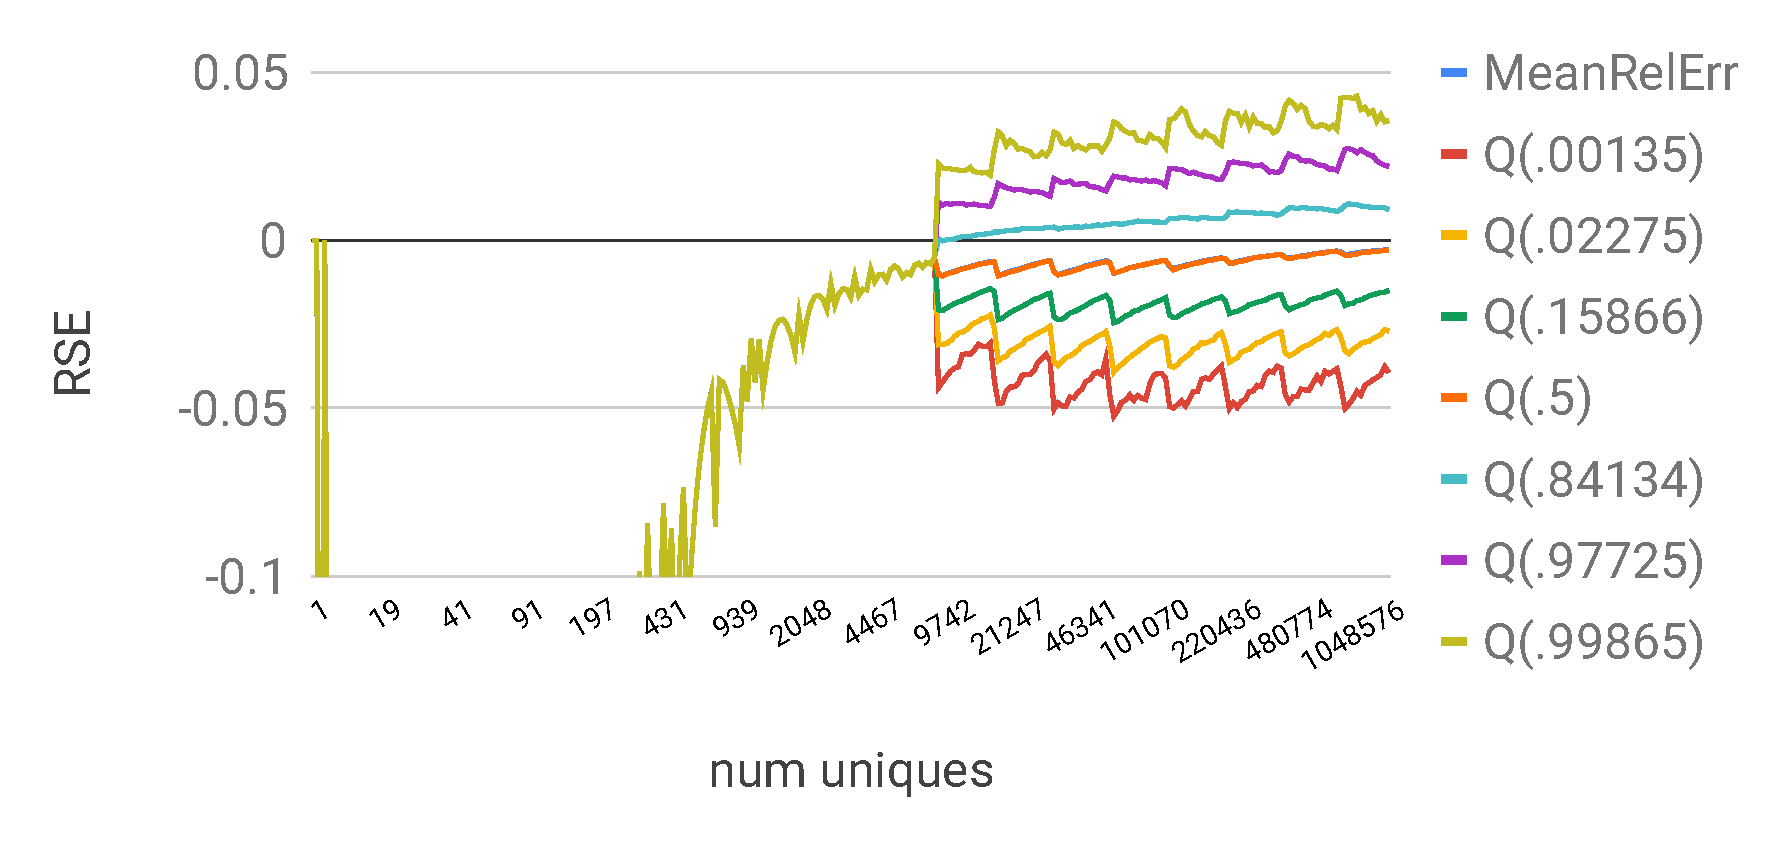
\includegraphics[width=\textwidth]{images/theta-accuracy.pdf}
    \caption{No eager propagation ($e=1.0$)}
    \label{fig:accuracy}
    \end{subfigure}
    \begin{subfigure}{\columnwidth}\centering
    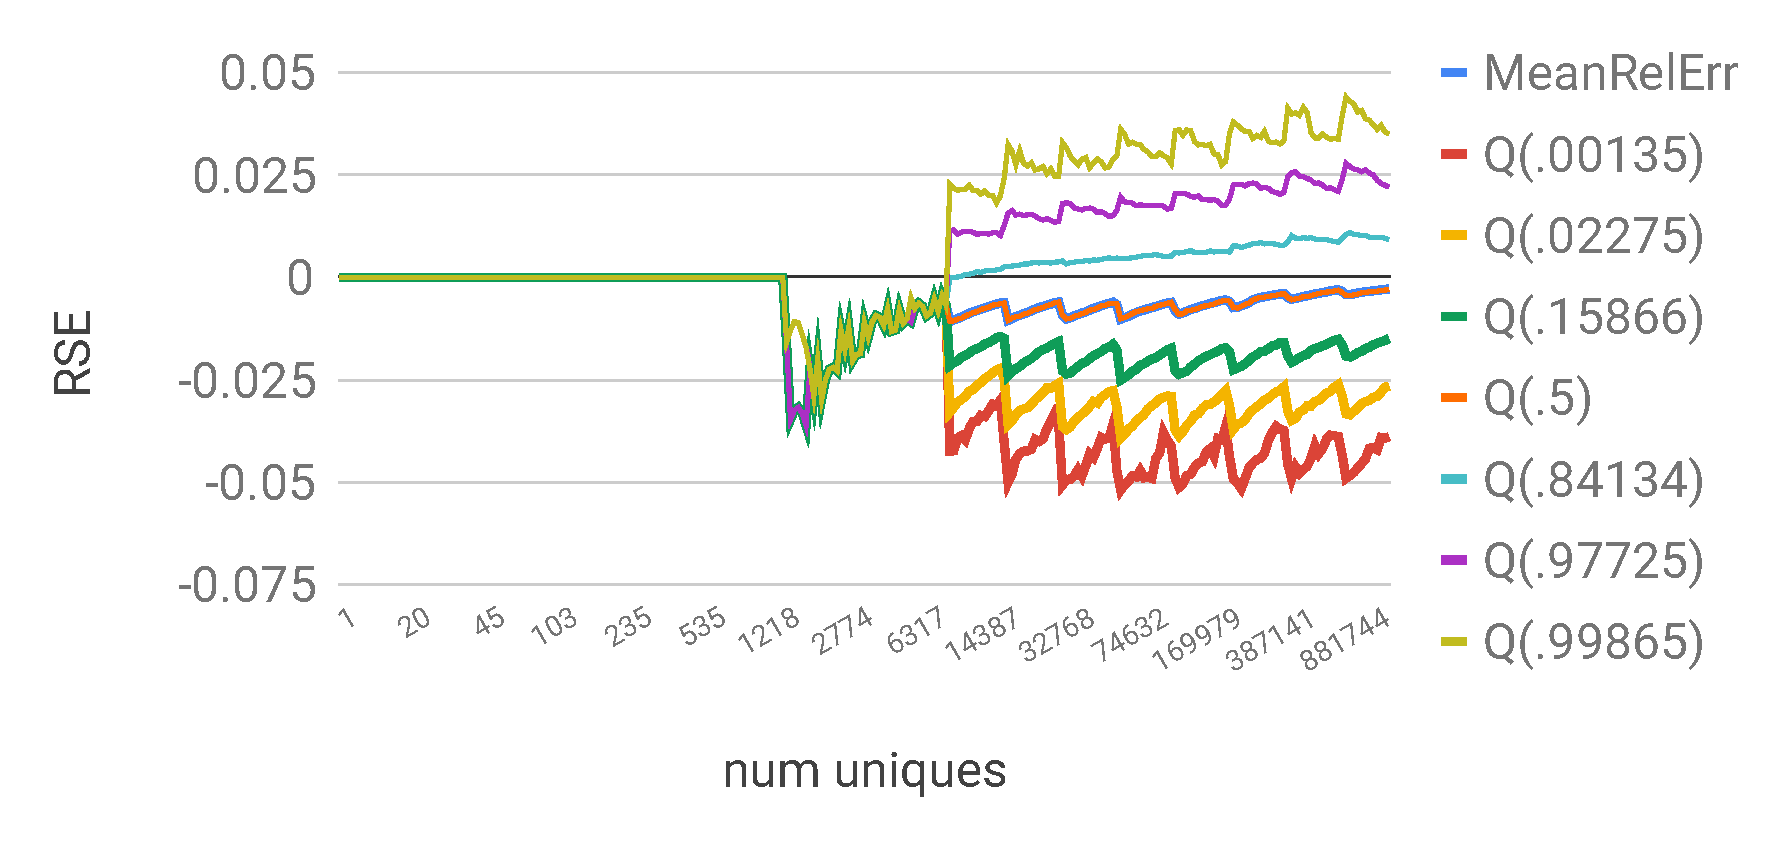
\includegraphics[width=\textwidth]{images/theta-accuracy-adaptive.pdf}
    \caption{With eager propagation, error bound defined by $e=0.04$}
    \label{fig:accuracy-adaptive}
    \end{subfigure}
      \caption{Concurrent $\Theta$ measured quantiles vs RSE, $k = 4096$.}
      \label{fig:accuracy-res}
\end{figure*}

\paragraph{Write-only workload}
Figure~\ref{fig:throughput:native} presents throughput measurements for a write-only workload. The results are shown in loglog scale.
Figure~\ref{fig:throughput:large} zooms-in on the throughput of large streams.

When considering large stream sizes, the concurrent implementation scales with the number of threads, peaking at
almost $300$M operations per second with $12$ threads. The performance of the lock-based implementation, on the other hand,
degrades as the contention on the lock increases. Its peak performance is
$25$M operations per second with a single thread. Namely, with a single thread, the concurrent $\Theta$ sketch outperforms the lock-based implementation
by $12$x, and with $12$ threads by more than $45$x. 

For small streams, wrapping a single thread with a lock is the most efficient method. Once the stream
contains more than $200$K unique values, using a concurrent sketch with $4$ or more local threads is more efficient.
The crossing point where a single local buffer is faster than the lock-based implementation is around $700$K unique values.
 
\begin{figure*}[tb]
\setlength{\abovecaptionskip}{0pt}
\setlength{\belowcaptionskip}{0pt}
\setlength\textfloatsep{0pt}
\centering
\begin{subfigure}{1.3\columnwidth}\centering
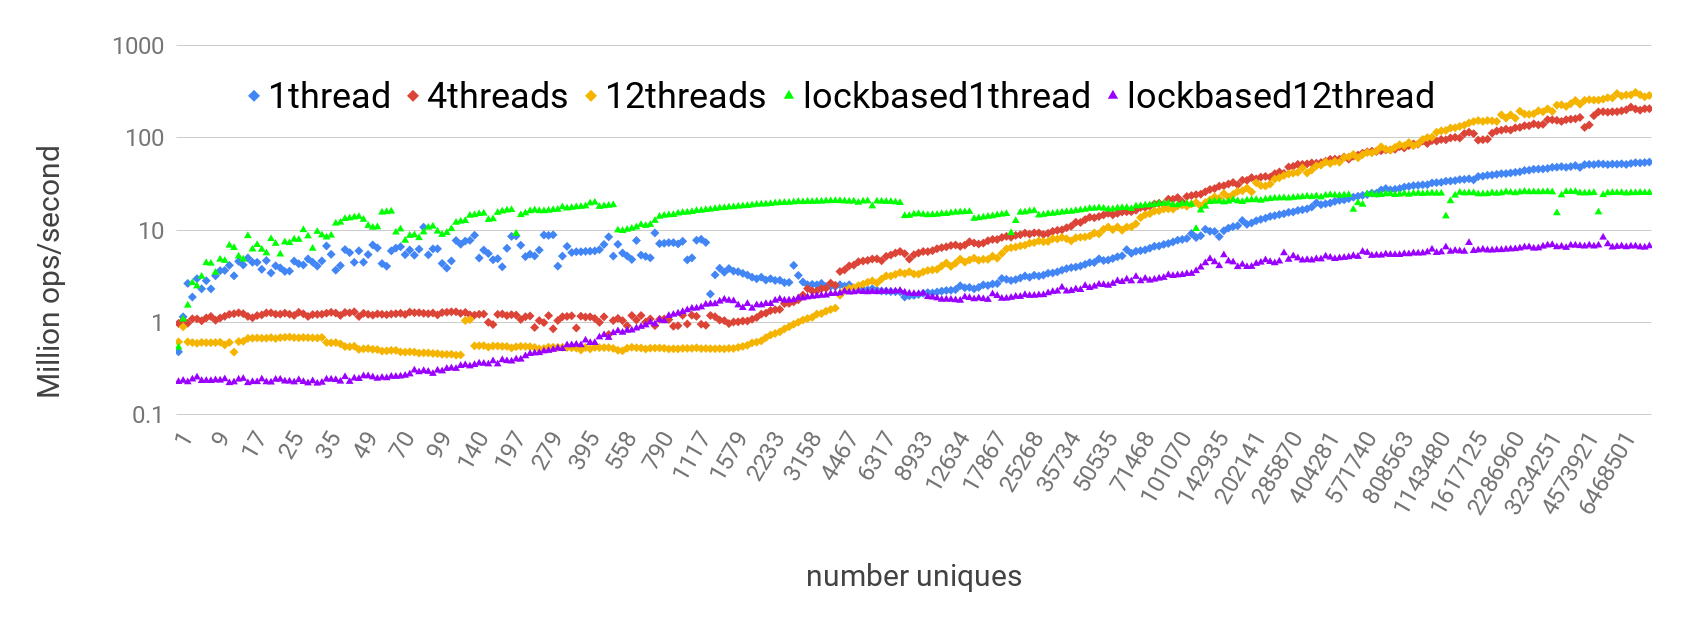
\includegraphics[width=\textwidth]{images/theta-write-only.png}
\caption{Throughput, loglog scale}
\label{fig:throughput:native}
\end{subfigure}
\begin{subfigure}{0.7\columnwidth}\centering
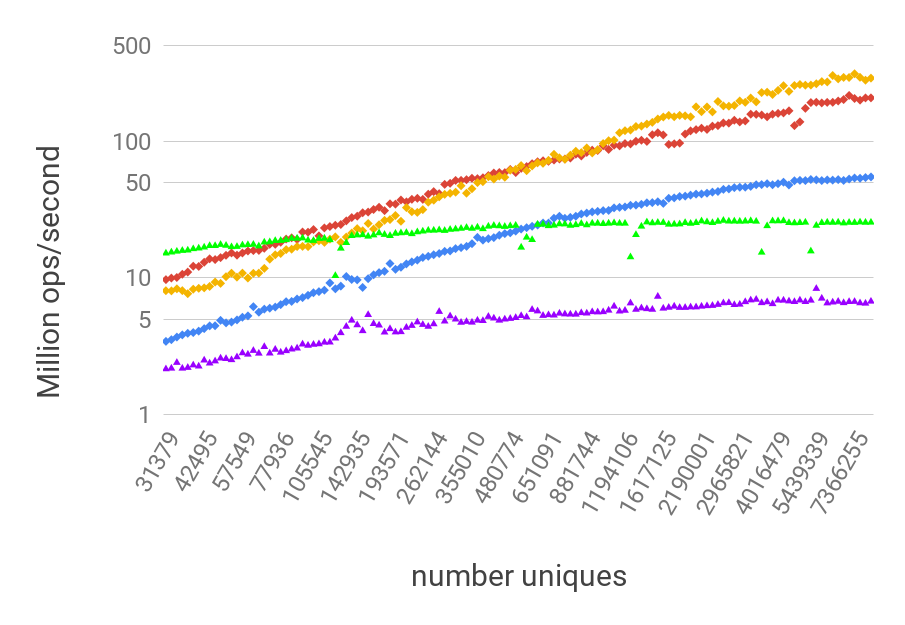
\includegraphics[width=\textwidth]{images/theta-write-only-zoomin.png}
\caption{Zooming-in on large sketches}
\label{fig:throughput:large}
\end{subfigure}
  \caption{Write-only workload, $k = 4096$, $e=0.04$.}
  \label{fig:throughput}
\end{figure*}


\paragraph{Mixed workload}
Figure~\ref{fig:mixed-throughput} presents the throughput measurements
of a mixed read-write workload. We compare runs with a single updating thread and $2$
updating threads (and $10$ background reader threads).
Although we see similar trends as in the write-only workload, the effect of
background readers is more pronounced in the lock-based implementation than in the concurrent one;
this is expected as the reader threads compete for the same lock as the writers.
The peak throughput of a single writer thread in the concurrent implementation is $55$M ops/sec both with and
without background readers. The peak throughput of a single writer thread in the lock-based
implementation degrades from $25$M ops/sec without background reads to $23$M ops/sec with them; this is an almost $10$\% slowdown in performance.
Recall that in this scenario reads are infrequent, and so the degradation is not dramatic.

\begin{figure}[tb]
\setlength{\abovecaptionskip}{0pt}
\setlength{\belowcaptionskip}{0pt}
\setlength\textfloatsep{0pt}
	\centering
	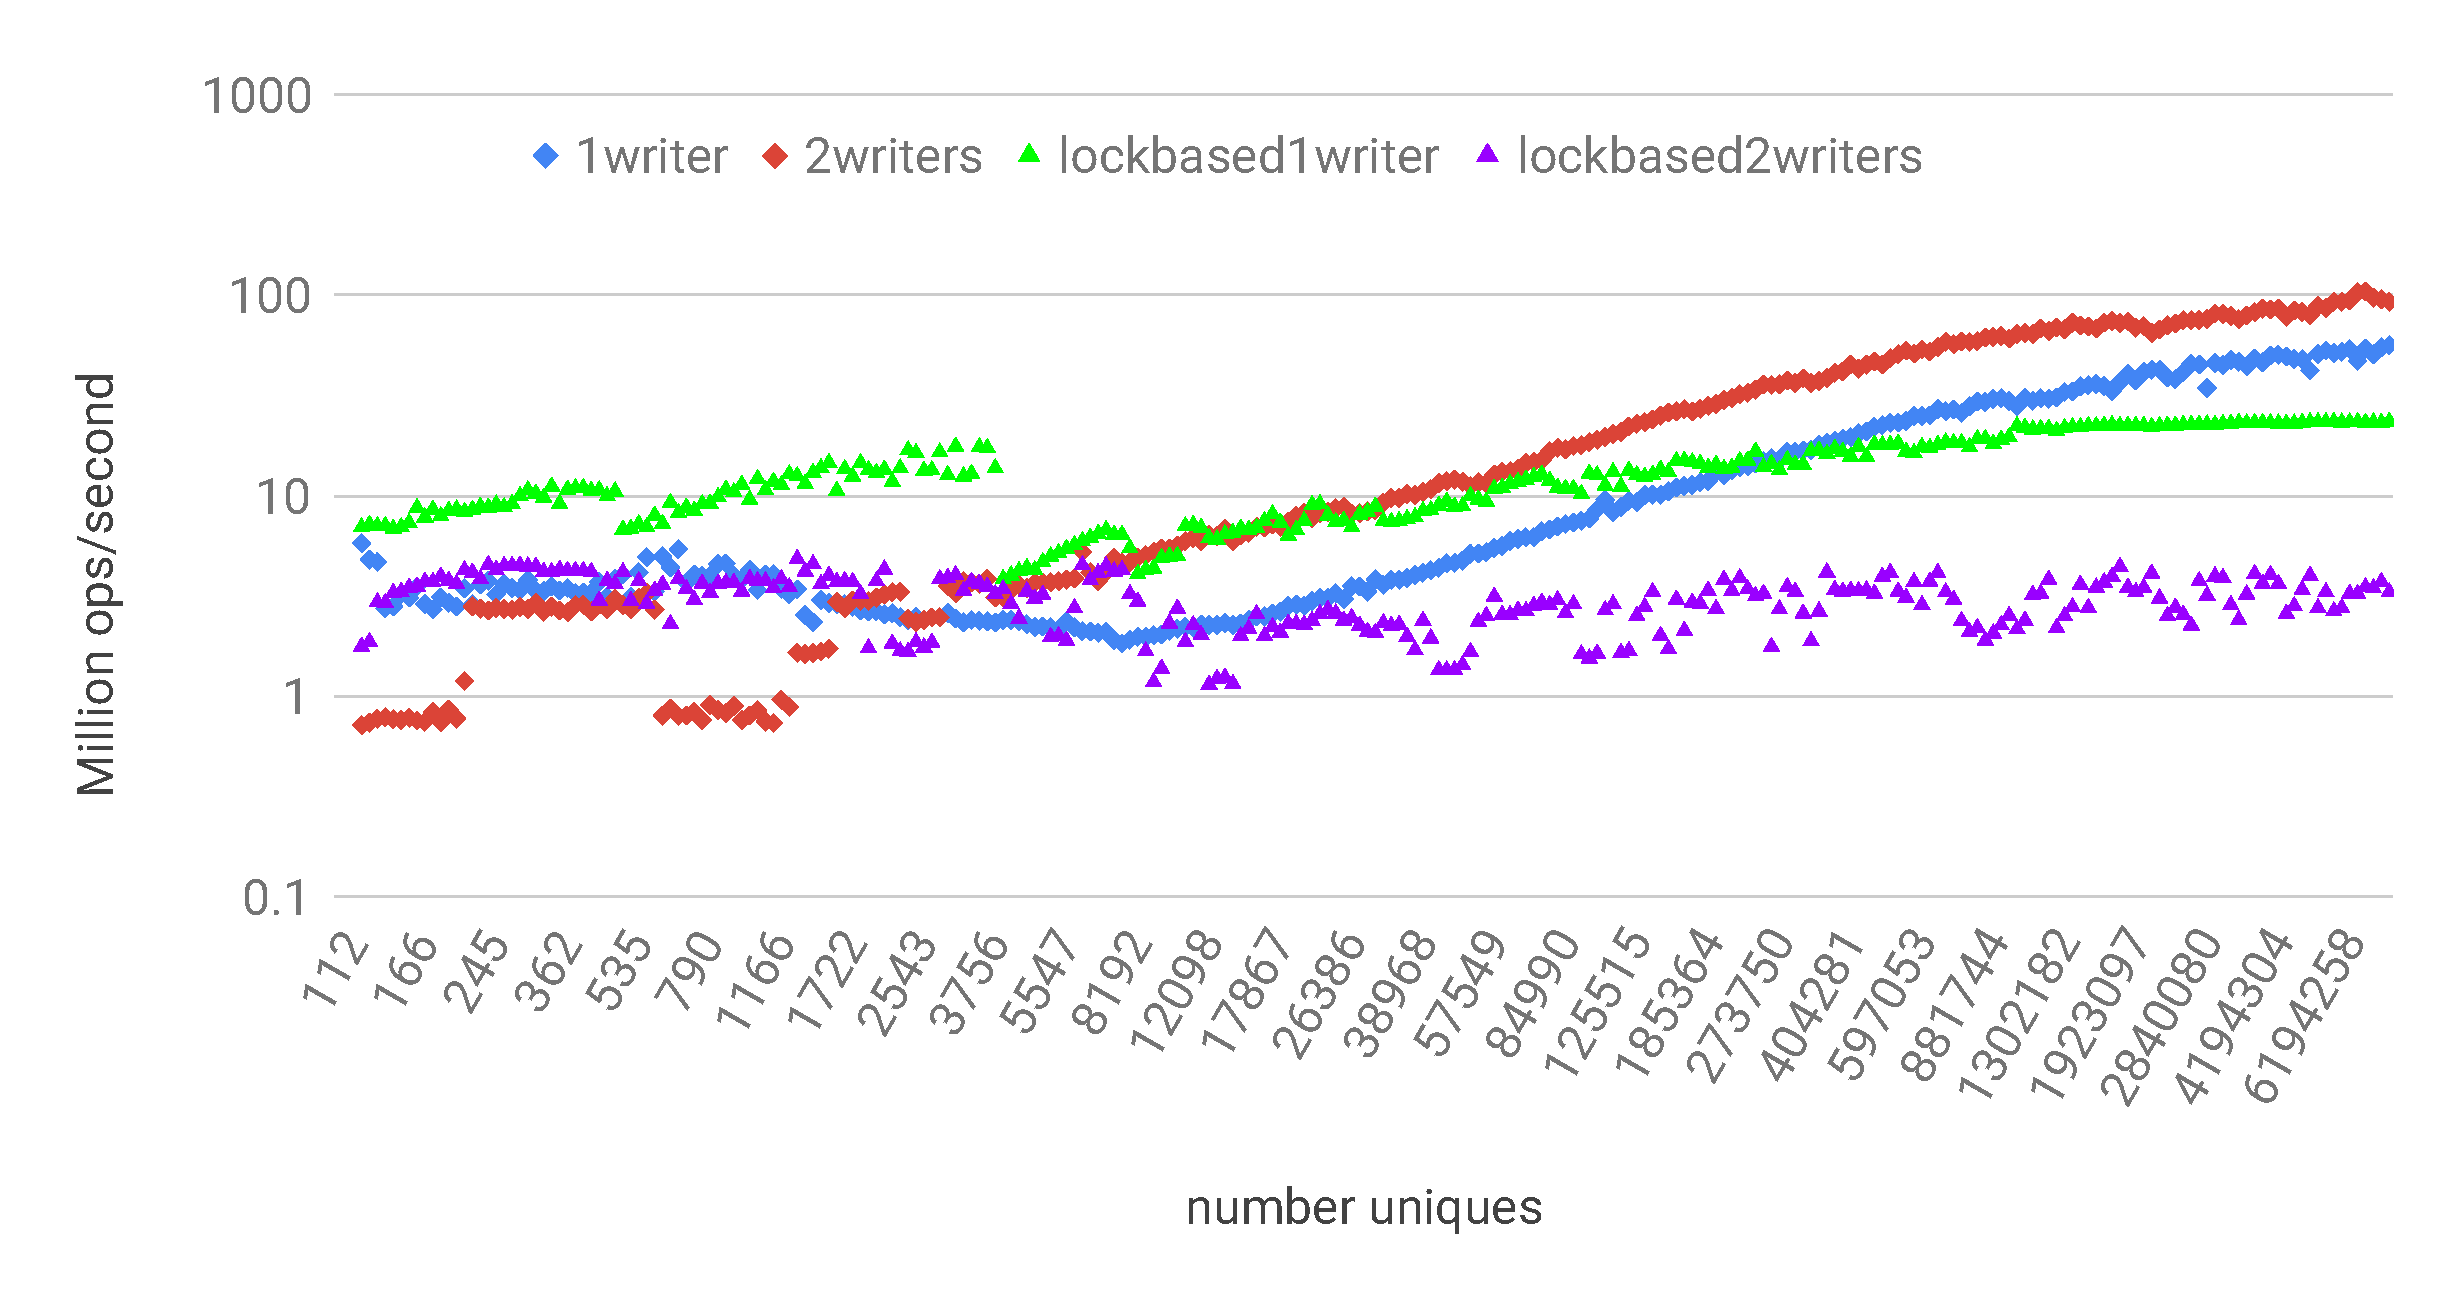
\includegraphics[width=\columnwidth]{images/theta-mixed.pdf}
	\caption{{Mixed workloads: writers with background reads, $k = 4096$, $e=0.04$.}}
	\label{fig:mixed-throughput}
\end{figure}


\paragraph{Scalability results}
To provide a better scalability analysis, we aim to maximize the number of threads working on the
sketch. Therefore, we run this test on a larger machine -- we use a 32-core Xeon E5-4650 processors.
We ran an \emph{update-only} workload in which a sketch is built from a very large stream, repeating
each test 16 times.

In Figure~\ref{fig:performance} (in the introduction) we compare the scalability
of our concurrent $\Theta$ sketch and the original sketch wrapped
with a read/write lock in an update-only workload, for $b=1$ and $k=4096$.
As expected, the lock-based sequential sketch does not scale, and
in fact it performs worse when accessed concurrently by many threads.
In contrast, our sketch achieves almost perfect scalability.
$\Theta$ quickly becomes small enough to allow filtering out most of the updates and so the
local buffers fill up slowly.


\subsection{Accuracy-throughput tradeoff}
\label{ssec:tradeoffs}

The speedup achieved by eager propagation in small streams is presented in Figure~\ref{fig:speedup}.
This is an additional advantage of eager propagation in small streams, beyond the accuracy benefit reported in Figure~\ref{fig:accuracy-res}. 
The improvement is as high as $84$x for tiny sketches, and tapers off as the sketch grows.
The slowdown in performance when the sketch size exceeds $2k$ can be explained by the reduction
in the local buffer size (from $b=16$ to $b=5$), needed in order to accommodate for the required error bound.

\begin{figure}[tb]
\setlength{\abovecaptionskip}{0pt}
\setlength{\belowcaptionskip}{0pt}
\setlength\textfloatsep{0pt}
	\centering
	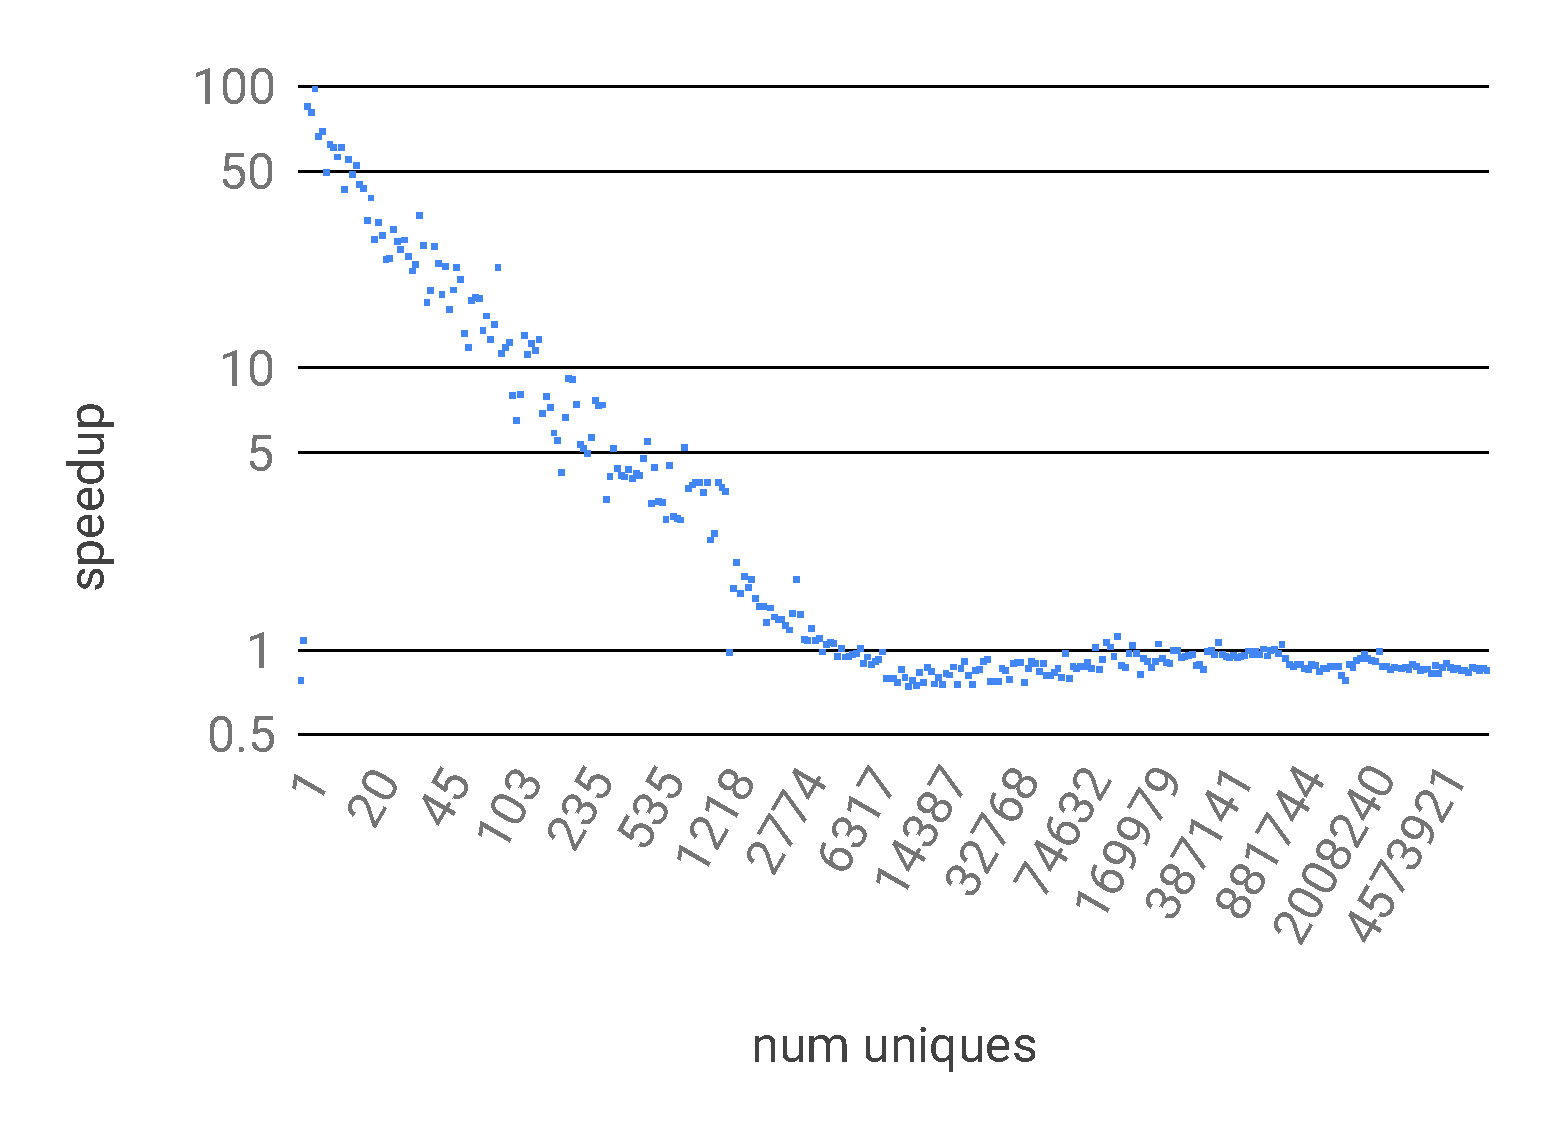
\includegraphics[width=\columnwidth]{images/eager-speedup.pdf}
	\caption{{Throughput speedup of eager ($e=0.04$) vs no-eager ($e=1.0$) propagation, $k = 4096$.}}
	\label{fig:speedup}
\end{figure}


Next we discuss the impact of $k$.
One way to increase the throughput of the concurrent $\Theta$ sketch is by
increasing the size of the global sketch, namely increasing $k$. On the other hand,
this change also increases the error of the estimate.
Table~\ref{tab:tradeoff} presents the tradeoffs between performance and accuracy.
Specifically, it presents the crossing-point, namely the smallest stream size for which the concurrent
implementation outperforms the lock-based implementation (both running a single thread). It further presents
the maximum values (across all stream sizes) of the median error and 99th percentile error for a variety of $k$ values.
The table shows that as the sketch promises a smaller error (by using a larger $k$), a larger stream size is needed to justify using
the concurrent sketch with all its overhead.

\begin{table}[htb]
\center{\small{
\begin{tabular}{lrrr}
\hline 
& thpt crossing point & mean error & error $Q=0.99$ \\
\hline 
$k=256$ &  15,000 &	0.16 & 0.27 \\
\hline 
$k=1024$ &  100,000 &	0.05 & 0.13 \\
\hline 
$k=4096$ & 700,000	& 0.03	& 0.05	\\ 
\hline 
\end{tabular}
}}
\caption{{Performance vs accuracy as a function of $k$.}}
\label{tab:tradeoff}
\end{table}  


